\apendice{Especificación de diseño}
\section{Clasificación de las asignaturas}
Se ha realizado una clasificación general de las áreas a las que pertenecen de forma general las  asignaturas, de forma que se pueda mostrar un gráfico en la materia recomendable para un alumno. La siguiente tabla hace referencia a dicha clasificación \ref{tab:C.1}
\begin{table}[]
\caption{Tabla áreas educativas de las asignaturas }
\label{tab:C.1}
\resizebox{\textwidth}{!}{
\begin{tabular}{ lrrrrrrrr }
\toprule
 & Matemáticas & Derecho & Programación & Algoritmos & Idiomas & Economía & Diseño & Equipos informáticos \\  
\textbf{PRIMER SEMESTRE} &  &  &  &  &  &  &  &  \\  
Fundamentos Deontológicos y Jurídicos de las TIC & 1 & 1 & 0 & 0 & 0 & 0 & 0 & 0 \\  
Álgebra Lineal & 1 & 0 & 0 & 0 & 0 & 0 & 0 & 0 \\  
Informática Básica & 0 & 0 & 1 & 0 & 0 & 0 & 0 & 0 \\  
Fundamentos Físicos de la Informática & 1 & 0 & 0 & 0 & 0 & 0 & 0 & 0 \\  
Matemática Discreta & 1 & 0 & 0 & 0 & 0 & 0 & 0 & 0 \\  
\textbf{SEGUNDO SEMESTRE} &  &  &  &  &  &  &  &  \\  
Inglés Aplicado a la Informática & 0 & 0 & 0 & 0 & 1 & 0 & 0 & 0 \\  
Cálculo & 1 & 0 & 0 & 0 & 0 & 0 & 0 & 0 \\  
Programación & 0 & 0 & 1 & 1 & 0 & 0 & 0 & 0 \\  
Fundamentos de los Computadores & 0 & 0 & 1 & 0 & 0 & 0 & 0 & 1 \\  
Sistemas Operativos & 0 & 0 & 1 & 1 & 0 & 0 & 1 & 1 \\  
\textbf{TERCER SEMESTRE} &  &  &  &  &  &  &  &  \\  
Metodología de la Programación & 0 & 0 & 1 & 1 & 0 & 0 & 0 & 0 \\ 
Estadística & 1 & 0 & 0 & 0 & 0 & 0 & 0 & 0 \\ 
Ingeniería del Software & 0 & 0 & 0 & 0 & 0 & 0 & 1 & 0 \\  
Bases de Datos & 0 & 0 & 1 & 0 & 0 & 0 & 1 & 0 \\  
Arquitectura de Computadores & 0 & 0 & 1 & 0 & 0 & 0 & 0 & 1 \\  
\textbf{CUARTO SEMESTRE} &  &  &  &  &  &  &  &  \\  
Estructuras de Datos & 0 & 0 & 1 & 1 & 0 & 0 & 0 & 0 \\  
Redes & 0 & 0 & 0 & 0 & 0 & 0 & 0 & 1 \\  
Interacción Hombre-Máquina & 0 & 0 & 1 & 0 & 0 & 0 & 1 & 0 \\  
Fundamentos de Organización y Gestión de Empresas & 0 & 0 & 0 & 0 & 0 & 1 & 0 & 0 \\  
Análisis y Diseño de Sistemas & 0 & 0 & 0 & 0 & 0 & 0 & 1 & 0 \\  
\textbf{QUINTO SEMESTRE} &  &  &  &  &  &  &  &  \\ 
Arquitecturas Paralelas & 0 & 0 & 1 & 0 & 0 & 0 & 0 & 1 \\ 
Sistemas Inteligentes & 0 & 0 & 1 & 1 & 0 & 0 & 1 & 0 \\ 
Gestión de Proyectos & 0 & 0 & 1 & 0 & 0 & 1 & 1 & 0 \\ 
Diseño y Administración de Sistemas y Redes & 0 & 0 & 0 & 0 & 0 & 0 & 0 & 1 \\  
Procesadores del Lenguaje & 0 & 0 & 1 & 1 & 0 & 0 & 0 & 0 \\  
\textbf{SEXTO SEMESTRE} &  &  &  &  &  &  &  &  \\ 
Programación Concurrente & 0 & 0 & 1 & 0 & 0 & 0 & 0 & 1 \\  
Seguridad Informática & 0 & 1 & 1 & 1 & 0 & 0 & 0 & 1 \\ 
Aplicaciones de Bases de Datos & 0 & 0 & 1 & 0 & 0 & 0 & 1 & 1 \\  
Algoritmia & 0 & 0 & 1 & 1 & 0 & 0 & 0 & 0 \\ 
Métodos Numéricos y Optimización & 1 & 0 & 1 & 0 & 0 & 0 & 0 & 0 \\  
\textbf{SÉPTIMO SEMESTRE} &  &  &  &  &  &  &  &  \\  
Diseño e Implementación de Sistemas Digitales & 0 & 0 & 1 & 0 & 0 & 0 & 1 & 1 \\ 
Gestión de la Información & 1 & 0 & 1 & 1 & 0 & 1 & 0 & 0 \\ 
Diseño y Mantenimiento del Software & 0 & 0 & 1 & 0 & 0 & 0 & 1 & 0 \\  
Organización y Gestión de Empresas & 0 & 0 & 1 & 1 & 0 & 1 & 0 & 0 \\  
 Mantenimiento de Equipos Informáticos & 1 & 0 & 0 & 0 & 0 & 0 & 0 & 1 \\  
Hardware de Aplicación Específica & 0 & 0 & 1 & 0 & 0 & 0 & 1 & 1 \\ 
Control por Computador & 0 & 0 & 1 & 0 & 0 & 0 & 0 & 1 \\ 
Validación y Pruebas & 0 & 0 & 1 & 1 & 0 & 0 & 1 & 0 \\
Computación Neuronal y Evolutiva & 0 & 0 & 1 & 1 & 0 & 0 & 0 & 0 \\ 
Programación de Sistemas Operativos & 0 & 0 & 1 & 0 & 0 & 0 & 0 & 1 \\ 
\textbf{OCTAVO SEMESTRE} &  &  &  &  &  &  &  &  \\ 
Sistemas Distribuidos & 0 & 0 & 1 & 1 & 0 & 0 & 1 & 0 \\ 
Sistemas Empotrados y de Tiempo Real & 0 & 0 & 1 & 0 & 0 & 0 & 0 & 1 \\
Métodos Formales & 1 & 0 & 1 & 0 & 0 & 0 & 1 & 0 \\ 
Nuevas Tecnologías y Empresa & 0 & 0 & 1 & 1 & 0 & 0 & 0 & 0 \\ 
Minería de Datos & 1 & 0 & 1 & 1 & 0 & 0 & 0 & 0 \\ 
Desarrollo Avanzado de Sistemas Software & 0 & 0 & 1 & 0 & 0 & 0 & 1 & 0 \\ \bottomrule
\end{tabular}
}
\end{table}


\section{Modelo de Interfaz Gráfica}
La interfaz gráfica de escritorio de la primera versión se realizará con PyQt5, de forma que habrá varias ventanas diferentes dependiendo de la funcionalidad seleccionada: 
\subsection{Inicio de Sesión}
En la primera pestaña al ejecutar la aplicación, se mostraría la pantalla de inicio sesión para introducir el correo y la contraseña. La siguiente imagen hace referencia a un modelo básico de la pantalla de inicio de sesión. ~\ref{fig:C.2.1}
\begin{figure}[h]
\centering
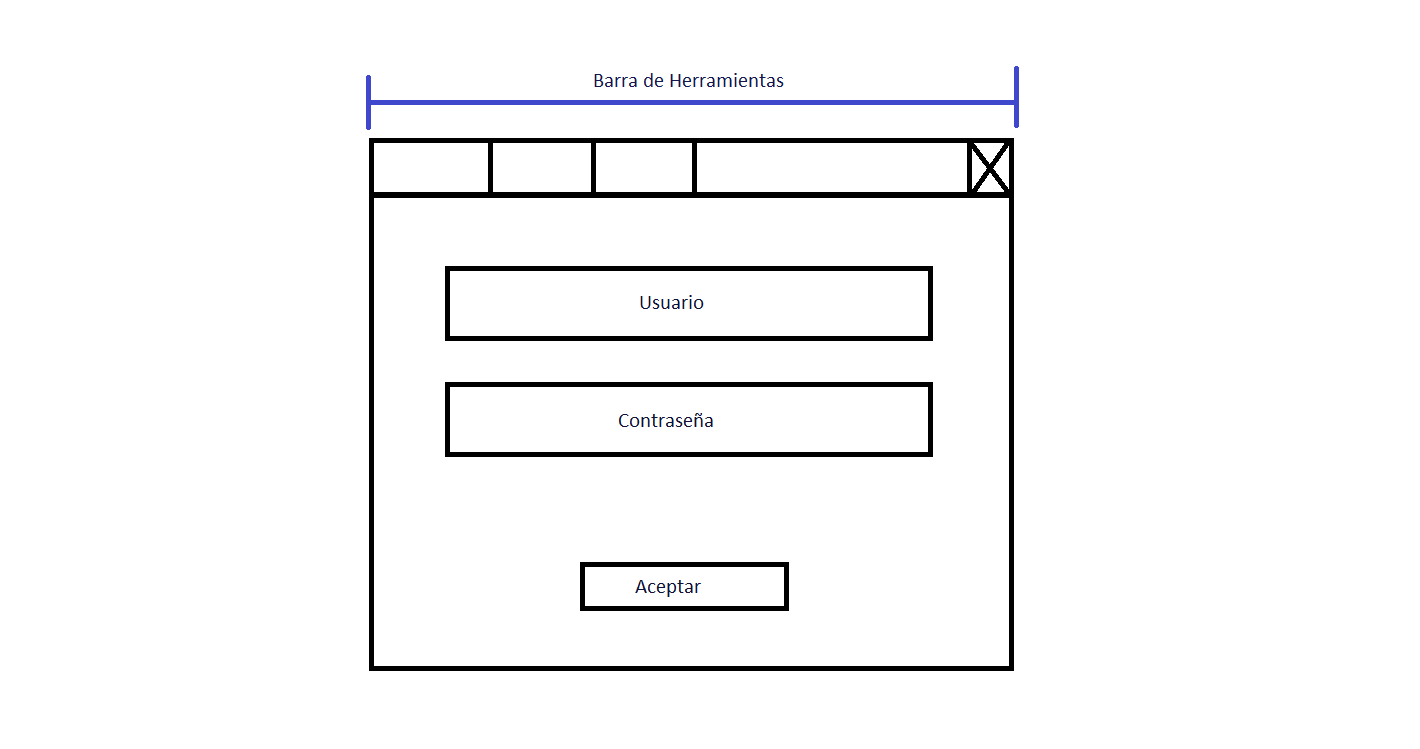
\includegraphics[width=0.90\textwidth]{PROTOTIPO_Inicio_sesion}
\caption{Prototipo de Inicio Sesión}
\label{fig:C.2.1}
\end{figure}

\subsection{Rellenado de cuestionario}
Una vez registrado por primera vez, un usuario debe rellenar el cuestionario con las ponderaciones de las asignaturas cursadas. Esta pestaña también sirve en caso de que el usuario se haya confundido en la calificación de alguna asignatura o repita el sistema de recomendación tras cursar nuevas asignaturas. Los diferentes cursos se seleccionarán en los botones para evitar un exceso de asignaturas mostradas en la pestaña. La siguiente imagen hace referencia a dicha pestaña. ~\ref{fig:C.2.2}
\begin{figure}[h]
\centering
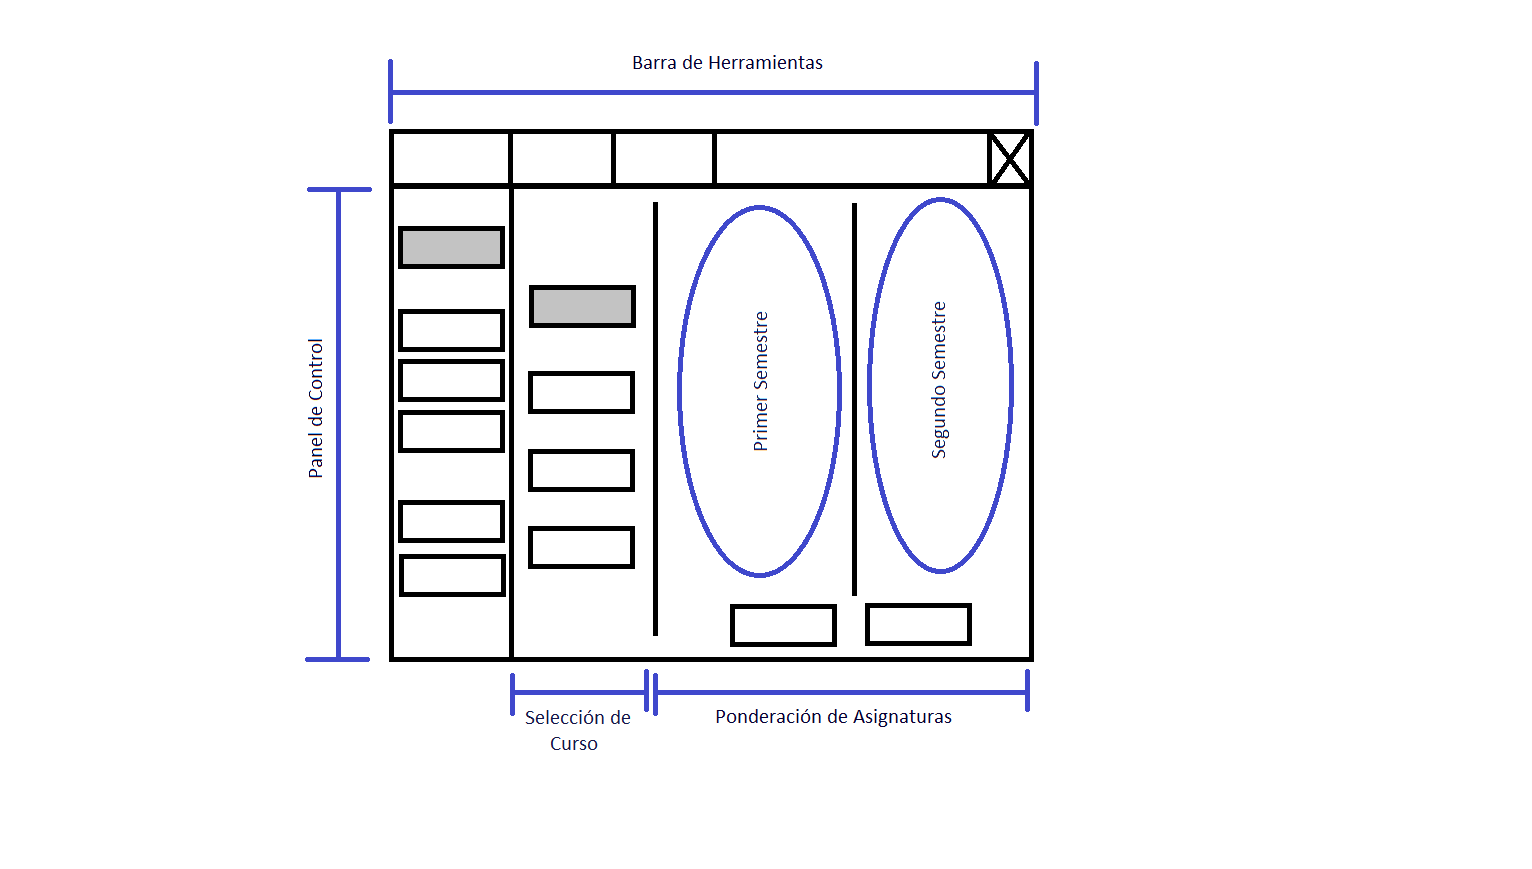
\includegraphics[width=0.90\textwidth]{PROTOTIPO_Rellenado_Datos}
\caption{Prototipo de Rellenado de datos}
\label{fig:C.2.2}
\end{figure}
\subsection{Muestra de resultados}
Tras rellenar el cuestionario para la recogida de datos, se seleccionará el sistema de recomendación deseado, y se mostrarán los resultados en base al sistema seleccionado, teniendo como patrón en el centro de la ventana los resultados de las asignaturas no cursadas, y en el tercio derecho, se mostrarán unas gráficas de las asignaturas y preferencias del alumno. La siguiente imagen hace referencia a dicha pestaña: ~\ref{fig:C.2.3}
\begin{figure}[h]
\centering
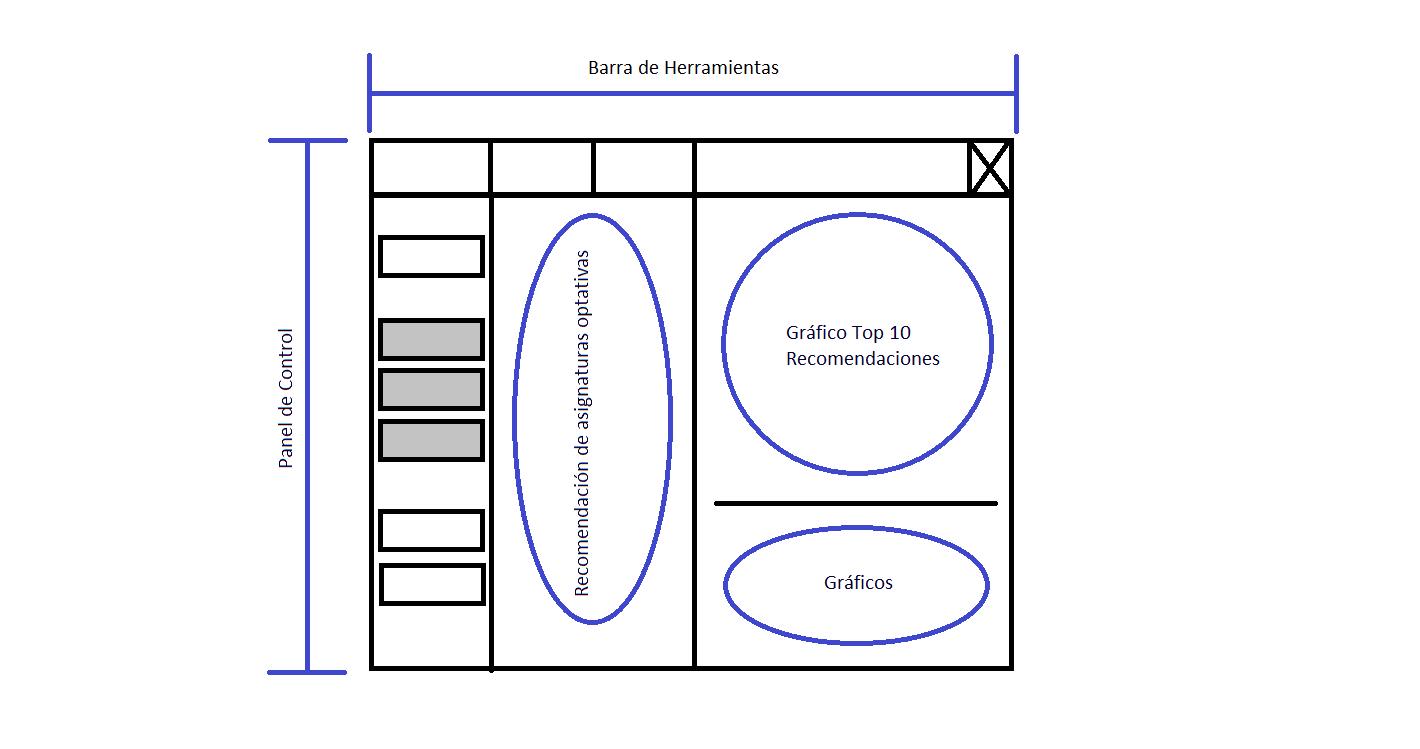
\includegraphics[width=0.90\textwidth]{PROTOTIPO_Sistemas_Recomendacion}
\caption{Prototipo de la muestra de datos}
\label{fig:C.2.3}
\end{figure}

\subsection{Otros datos}
Habrá un botón adicional que muestre las preferencias generales de media de los usuarios, así como otras gráficas para información adicional al usuario. 
La siguiente imagen hace referencia a dicha pestaña: ~\ref{fig:C.2.4}
\begin{figure}[h]
\centering
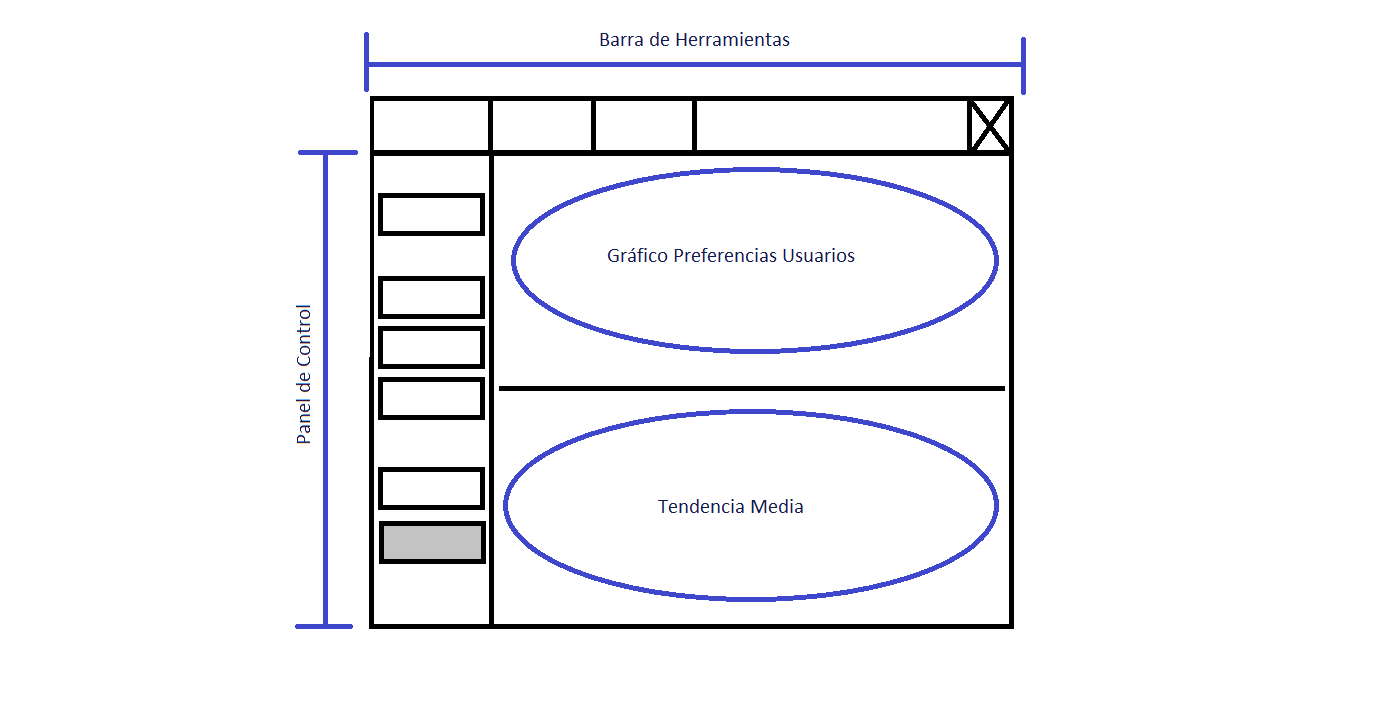
\includegraphics[width=0.90\textwidth]{PROTOTIPO_Otros_Datos}
\caption{Prototipo de datos adicionales}
\label{fig:C.2.4}
\end{figure}

\section{Diseño de Interfaz Gráfica }
\subsection{Inicio de Sesión}
La interfaz de inicio de sesión de la primera versión ~\ref{fig:C.3.1}  permite introducir el usuario y la contraseña en caso de estar registrado. En caso contrario, se debe pulsar "Registrarse" para crear una nueva cuenta. 
\begin{figure}[h]
\centering
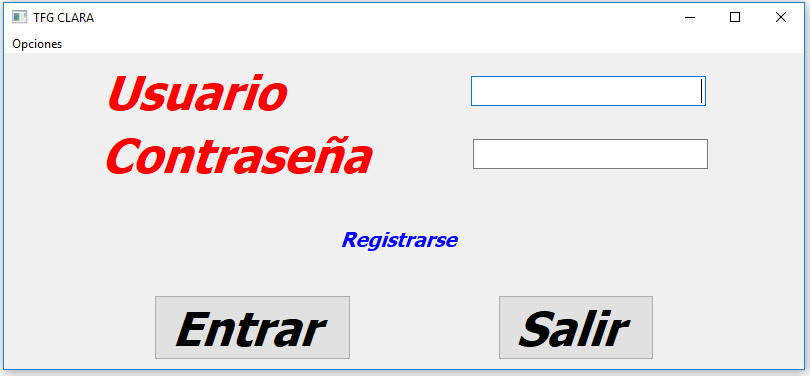
\includegraphics[width=0.90\textwidth]{INTERFAZ_Inicio_sesion}
\caption{Interfaz de inicio sesión}
\label{fig:C.3.1}
\end{figure}

\subsection{Rellenado de cuestionario}
Tras iniciar sesión, se mostrará la siguiente pestaña ~\ref{fig:C.3.2} en la que el usuario debe ponderar las asignaturas cursadas, siendo las del primer curso obligatorias para la ejecución del sistema de recomendación. 
\begin{figure}[h]
\centering
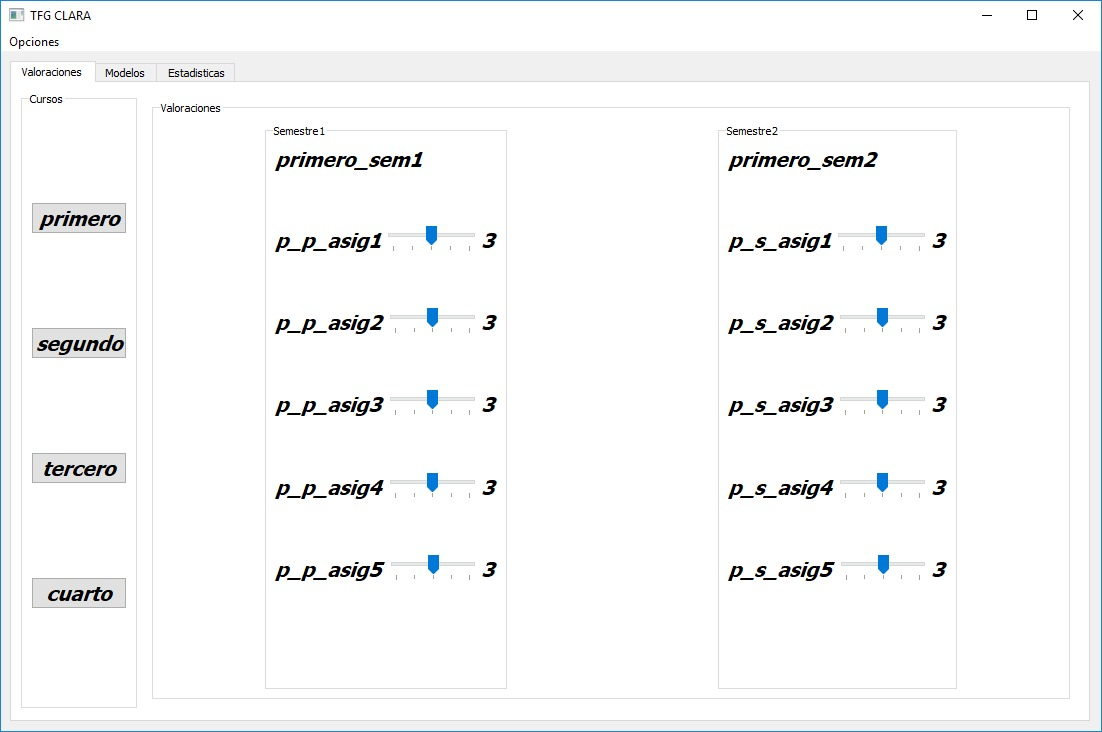
\includegraphics[width=0.90\textwidth]{INTERFAZ_Rellenado_Datos}
\caption{Interfaz de rellenado de cuestionario}
\label{fig:C.3.2}
\end{figure}

\subsection{Muestra de resultados}
Tras el rellenado de datos, se habilitan los botones de la selección del sistema de recomendación, mostrándose una pestaña similar a la siguiente: ~\ref{fig:C.3.3}
\begin{figure}[h]
\centering
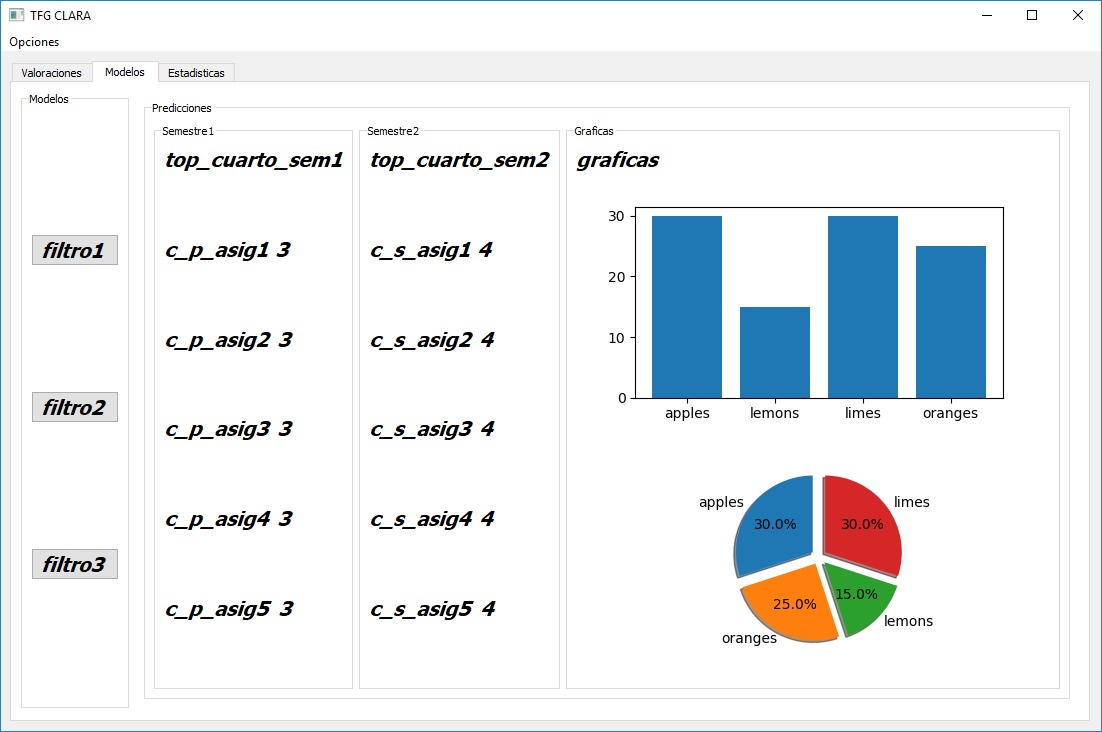
\includegraphics[width=0.90\textwidth]{INTERFAZ_Sistemas_Recomendacion}
\caption{Interfaz de la muestra de datos}
\label{fig:C.3.3}
\end{figure}

\subsection{Otros datos}
Se le mostrará unos datos auxiliares al usuario, en forma de gráficas, para mejorar su comprensión. Esto corresponde a la tercera pestaña de la aplicación. ~\ref{fig:C.3.4}
\begin{figure}[h]
\centering
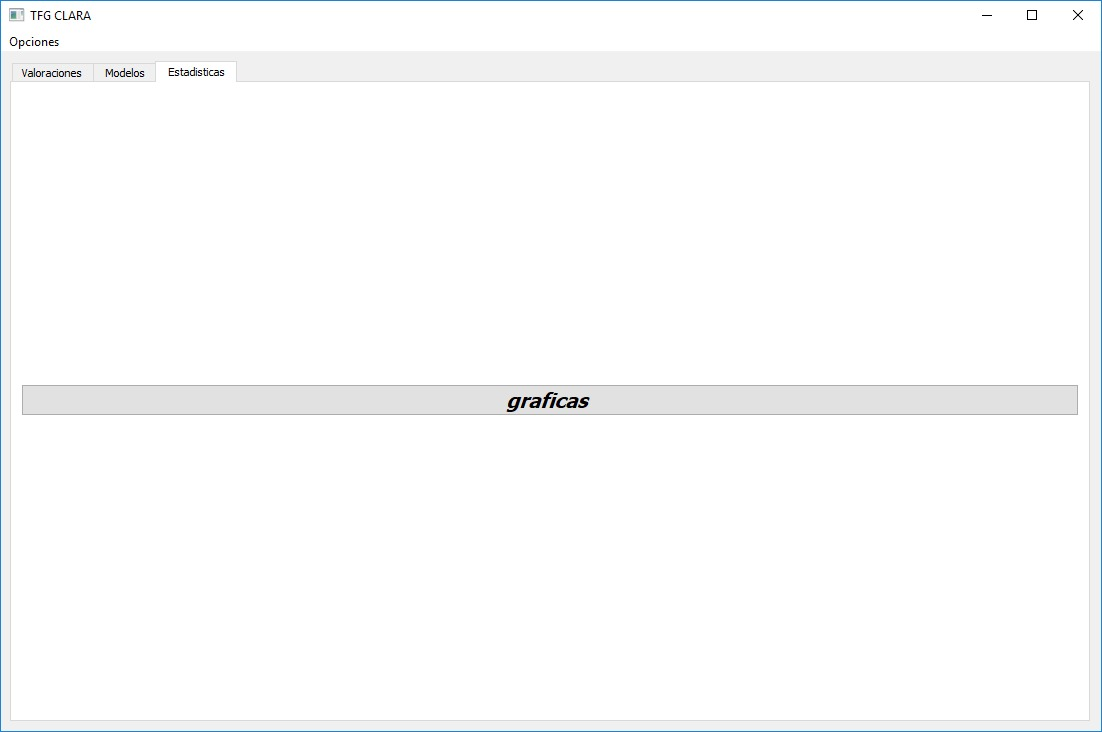
\includegraphics[width=0.90\textwidth]{INTERFAZ_Otros_datos}
\caption{Interfaz de datos adicionales}
\label{fig:C.3.4}
\end{figure}

\section{Posibles acciones del Usuario}
A continuación se detallarán las posibles acciones que se le permite realizar a un usuario: 
\subsection{Pestaña de Inicio}
En la pestaña de inicio, se permite a un usuario: 
\begin{itemize}
\item \textbf{Registrarse}: Al registrarse,-recibiendo el rol de Usuario y nunca de Admin- se le solicitará: 
\begin{itemize}
\item Nombre
\item Correo
\item Contraseña
\end{itemize}	

\item \textbf{Iniciar Sesión}: Al iniciar sesión se le solicitará  al usuario el usuario y la contraseña, validándose que los datos sean correctos.
\item \textbf{Salir}: Al pulsar el botón salir, se cerrará la pestaña, al igual si pulsa la X de la esquina superior derecha. 
\item \textbf{Aceptar}: Tras rellenar correctamente Usuario y Contraseña, se pulsará el botón aceptar para iniciar sesión y acceder a la aplicación. 
\end{itemize}


\subsection{Rellenado de Datos}
El primer botón de la pestaña superior permite acceder al rellenado de los datos para obtener las calificaciones de las asignaturas no cursadas. En caso de no haberse rellenado el mínimo necesario de las asignaturas, el resto de los botones, en la pestaña de selección del sistema de recomendación, exceptuando "Salir" permanecerán desactivados. 
La interacción que se le permite al usuario en dicha pestaña será la siguiente. 
\begin{itemize}
\item \textbf{Selección del curso}: Selección del curso para rellenar los datos. 
\item \textbf{Ponderación de asignatura}: Se permite ponderar en un Spiner tanto con el ratón, como con el teclado.
\item \textbf{Guardar}: Guardar los datos insertados  manualmente  por el usuario. 
\item \textbf{Modificación}: Se permitirá al usuario modificar las calificaciones en caso de haber insertado incorrectamente la ponderación. 

\end{itemize}

\subsection{Selección del sistema de Recomendación}
La selección del sistema de recomendación se realiza en la segunda pestaña de la aplicación. En dicha pestaña, habrá botones que  estarán deshabilitados hasta que el usuario complete el rellenado mínimo de los datos. 
La interacción que se le permite-tras habilitarse-será la siguiente: 
\begin{itemize}
\item Seleccionar el sistema de recomendación. 
\end{itemize}

\subsection{Muestra de otros datos}
La tercera pestaña hacer referencia  a la muestra de datos al usuario. Para ello, en un principio, no se le añadirá funcionalidad auxiliar al usuario.


\section{Posible diseño de Clases} 
El paquete Core,  en el que se encontrará toda la estructura de los sistemas de recomendación, se subdivide en dos paquetes diferentes: I\_O (de entrada y salida de datos) y Filtros (para el desarrollo de los sistemas de recomendación). La siguiente imagen corresponde con dicho esquema. 
 ~\ref{fig:C.3.5}
\begin{figure}[h]
\centering
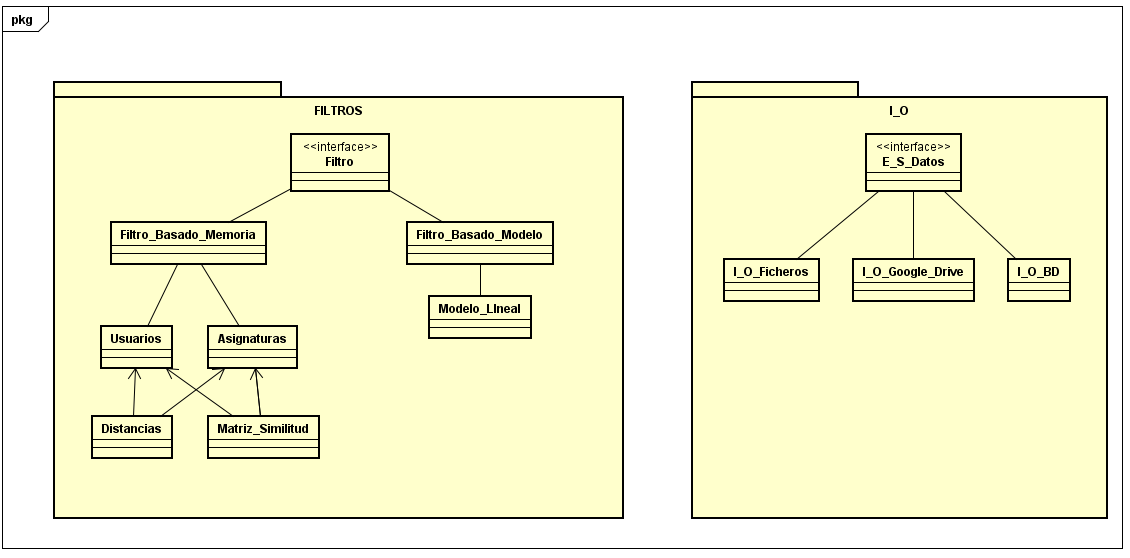
\includegraphics[width=0.90\textwidth]{Diagrama_Core}
\caption{Diagrama de Clases del Core}
\label{fig:C.3.5}
\end{figure}